\documentclass{article}

\usepackage[top=3cm, bottom=3cm, left=3cm, right=3cm]{geometry}

\usepackage[utf8]{inputenc}
\usepackage[T1]{fontenc}
\usepackage[frenchb]{babel}

\usepackage[a4paper,colorlinks,linkcolor=darkgray,citecolor=red,urlcolor=blue]{hyperref}
\usepackage{graphicx}
\usepackage{caption}
\usepackage{subcaption}
\usepackage{amsthm}
\usepackage{listings}
\usepackage{tikz}
\usepackage{algorithm}
\usepackage{amsmath}
\usepackage[noend]{algpseudocode}
\usepackage{amsfonts}
\usepackage{amssymb}
\usepackage{authblk}

\usepackage{tikz} % Let us start the fun
\usetikzlibrary{positioning, chains, calc, arrows, decorations.pathreplacing, fit, patterns, snakes}

\theoremstyle{definition} 
\newtheorem{definition}{Définition} 

\makeatletter
 
\newskip\@bigflushglue \@bigflushglue = -100pt plus 1fil
 
\def\bigcenter{\trivlist \bigcentering\item\relax}
\def\bigcentering{\let\\\@centercr\rightskip\@bigflushglue%
\leftskip\@bigflushglue
\parindent\z@\parfillskip\z@skip}
\def\endbigcenter{\endtrivlist}
 
\makeatother

\renewcommand\Affilfont{\small}

\title{Projet Images}

\author[$\dag$]{Laureline Pinault et Raphaël Charrondière}
\affil[$\dag$]{ENS de Lyon, France}

\date{Lundi 4 mai 2015}

\begin{document}

  \maketitle

  \begin{abstract}
	Laureline Pinault et Raphaël Charrondière sont fiers de vous présenter leur classificateur d'images !
  \end{abstract}
  
  \newpage

  \tableofcontents

  \newpage
  
  \section{Introduction}

    \subsection{Objectifs du projet}
    	Ce projet a pour but de coder un classificateur d'images en noir et blanc. Un classificateur d'images est un programme qui étant donné une image en entrée renvoie sa classe. Une classe représente un objet. Par exemple une image peut appartenir à la classe pomme si elle représente une pomme.

    \subsection{Remarques préliminaires}    	
    	Ce projet est réalisé en c++  et s'appuie sur la bibliothèque DGtal.
    	  
  \section{Organisation du projet} %TODO : Raphaël
  	Ce projet a été réalisé de manière très modulaire. Il ne s'agit pas d'un classificateur unique, mais de petits classificateurs qui combinés deviennent à priori plus précis. Ainsi le choix a été fait de créer des bibliothèques chargées dynamiquement par le programme central qui les exécute les uns après les autres. L'avantage de procéder ainsi est de cloisonner chaque classificateur (que l'on appellera aussi estimateur) afin qu'aucun n'infère sur l'autre. En particulier si l'un dysfonctionne il ne perturbe pas le déroulement du programme ou il suffit juste le supprimer.
  	   
  	   \subsection{Estimateur, comment ça fonctionne}
	Un classificateur ne renvoie pas directement une classe, en fait il va comparer un modèle à une image et dire selon lui comment le modèle et l'image sont éloignés. Du point de vue extérieur un estimateur comporte trois fonctions : \verb-buildmodel-, \verb-pre_estim- et \verb-estim-. La première donne une liste de fichier d'une même classe et renvoie un modèle, celui-ce pouvant être quelconque (un entier ou un graphe par exemple). La deuxième demande de réduire l'image à une donnée, la motivation étant de pouvoir rapidement comparer cette donnée à plusieurs modèles, cette comparaison étant faite par la troisième fonction qui renvoie un score $sc \in [0,1]$ de ressemblance approchant 1 quand elle est certaine ou 0 si le modèle ne correspond pas.

  	   \subsection{Classifions}
  	   Une fois que les modèles sont générés, la classification est facile. Pour chaque classe on considère les modèles de chaque classificateur, puis moyenne les scores qu'ils renvoient, ce qui détermine le score d'appartenance à cette classe. La signature d'une image est définie comme la concaténation de ces scores dans un vecteur. Le programme peut soit renvoyer cette signature, soit afficher les classes dont le score d'appartenance est supérieur à 0.9, soit rendre la classe ayant le plus haut score.
  	   
  	    Les modèles sont sauvegardés dans une base de données SQlite3 nommée \verb-estimatormodels.db-. Ils ont tous été générés. Il est à noter que la durée de construction de ces modèles est d'environ une à deux heures.
  
  \section{Traitement des images}
  
  	Il est à noter que les traitements sur images ne sont pas systématiquement appliqués. Chaque estimateur peut l'appliquer s'il en a besoin, selon la résistance au bruit, à l'agrandissement d'image, etc.
  
    \subsection{Traitement anti-inversion}
    \label{sec:anti-inversion}
    
      \begin{figure}[!h]
	\centering
	\begin{subfigure}{.49\textwidth}
	  \begin{subfigure}{.49\textwidth}
	    \centering
	    \includegraphics[scale=0.25]{Illustrations/rat-8.png}
	    \label{1strat}
	  \end{subfigure}
	  \begin{subfigure}{.49\textwidth}
	    \centering
	    \includegraphics[scale=0.25]{Illustrations/rat-8-inverse.png}
	    \label{1strat-inverse}
	  \end{subfigure}
	  \subcaption{Ce rat n'a pas été inversé}
	\end{subfigure}
	\begin{subfigure}{.49\textwidth}
	  \begin{subfigure}{.49\textwidth}
	    \centering
	    \includegraphics[scale=0.25]{Illustrations/rat-9.png}
	  \label{2ndrat}
	  \end{subfigure}
	  \begin{subfigure}{.49\textwidth}
	    \centering
	    \includegraphics[scale=0.25]{Illustrations/rat-9-inverse.png}
	  \label{2ndrat-inverse}
	  \end{subfigure}
	  \subcaption{Ce rat a été inversé}
	\end{subfigure}
	\caption{Inversion de l'objet rat}
	\label{anti-inversion}
      \end{figure}

    \subsection{Normalisation des images}  
    
    Cette opération consiste d'abord à calculer le centre de gravité $G$ de l'objet, puis à calculer l'éloignement moyen $m$ à celui-ci, c'est à dire le distance moyenne point de l'objet à son centre de gravité.
    
    Ensuite, on crée un nouvelle image d'une taille $800 \times 800$ correspondant à l'image recentrée en G affichant les points d'origines de la fenêtre de taille $4m \times 4m$.
    
    Cela permet d'avoir un objet normé en taille et centré (donc est idéal pour des estimateurs travaillant sur l'aire ou sensible aux translations).
      
    \subsection{Traitement anti-bruit}
    \label{sec:anti-bruit}
    
    On utilisera ici un traitement basique. Il s'agit juste de re-colorier un pixel par la couleur majoritaire chez ses huit voisins. Une passe peut corriger le bruit, mais itérer les passes jusqu'à la stabilité donne de meilleur résultats comme montré sur les figures ci dessous (en majorant par huit itérations pour assurer la terminaison et borner le temps d'exécution).
    
     \begin{figure}[!h]
	\centering
	  \begin{subfigure}{.24\textwidth}
	    \centering
	    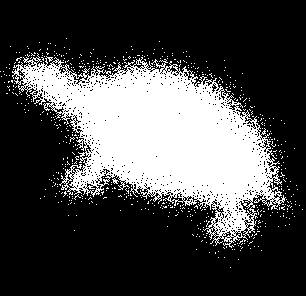
\includegraphics[scale=0.3]{Illustrations/turtle-1-bruit.png}
	    \label{butterfly-rempli}
	  \end{subfigure}
	  \begin{subfigure}{.24\textwidth}
	    \centering
	    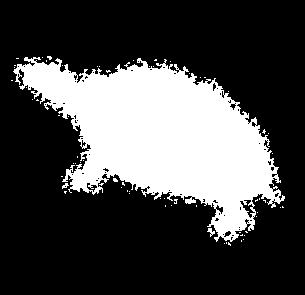
\includegraphics[scale=0.3]{Illustrations/turtle-1-bruit1.png}
	    \label{spirale-rempli}
	  \end{subfigure}
	  \begin{subfigure}{.24\textwidth}
	    \centering
	    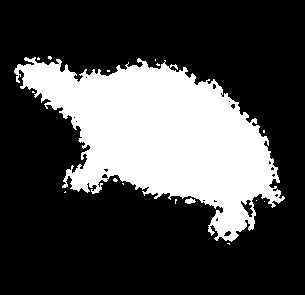
\includegraphics[scale=0.3]{Illustrations/turtle-1-bruit2.png}
	  \label{1stcup-rempli}
	  \end{subfigure}
	  \begin{subfigure}{.24\textwidth}
	    \centering
	    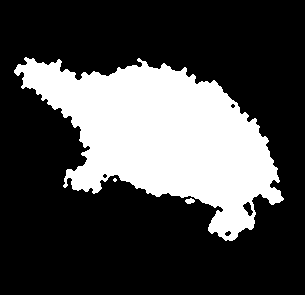
\includegraphics[scale=0.3]{Illustrations/turtle-1-bruitf.png}
	  \label{2ndcup-rempli}
	  \end{subfigure}
	\caption{Le traitement contre le bruit : dans l'ordre l'image originale, l'image corrigée une fois, puis deux, puis jusqu'à stabilité}
	\label{Traitement-Bruit}
    \end{figure}
    
    \subsection{Remplissage}
    \label{sec:remplissage}
    
      \begin{figure}[!h]
	\centering
	\begin{subfigure}{.25\textwidth}
	  \centering
	  \includegraphics[scale=0.30]{Illustrations/pocket-20.png}
	  \label{pocket-non-rempli}
	\end{subfigure}
	\begin{subfigure}{.25\textwidth}
	  \centering
	  \includegraphics[scale=0.30]{Illustrations/pocket-20-rempli.png}
	\label{pocket-rempli}
	\end{subfigure}
	\caption{Remplissage de l'objet pocket}
	\label{remplissage}
      \end{figure}
      
      \begin{figure}[!h]
	\centering
	\begin{subfigure}{.47\textwidth}
	  \begin{subfigure}{.52\textwidth}
	    \centering
	    \includegraphics[scale=0.295]{Illustrations/butterfly-10-rempli.png}
	    \label{butterfly-rempli}
	  \end{subfigure}
	  \begin{subfigure}{.45\textwidth}
	    \centering
	    \includegraphics[scale=0.16]{Illustrations/device9-6-rempli.png}
	    \label{spirale-rempli}
	  \end{subfigure}
	  \subcaption{Certains détails ne sont pas remplis}
	\end{subfigure}
	\begin{subfigure}{.44\textwidth}
	  \begin{subfigure}{.46\textwidth}
	    \centering
	    \includegraphics[scale=0.25]{Illustrations/cup-7-rempli.png}
	  \label{1stcup-rempli}
	  \end{subfigure}
	  \begin{subfigure}{.46\textwidth}
	    \centering
	    \includegraphics[scale=0.275]{Illustrations/cup-12-rempli.png}
	  \label{2ndcup-rempli}
	  \end{subfigure}
	  \subcaption{Les tasses ne sont pas remplies pareil}
	\end{subfigure}
	\caption{Problèmes soulevés par le remplissage des objets}
	\label{problèmes-remplissage}
      \end{figure}      
   
  \section{Estimateurs}
  
    \subsection{Estimateurs et modèles}
    
    Tout les estimateurs ici renvoient une grandeur caractéristique (ou deux). La construction du modèle consiste juste à calculer la moyenne $m$ et l'écart-type de ce scalaire $v$ . Ensuite le score d'une image est défini par : $ \sqrt[4]{\exp{\left (-\frac{(x-m)^4}{2v}\right )}}$si $x$ est sa valeur caractéristique. Si il y a deux valeurs caractéristiques, on multipliera juste le score des deux.
  
    \subsection{Quelques estimateurs simples et complémentaires}

      Une première idée fut de travailler sur la forme générale de la forme \textendash est-ce qu'elle est plutôt carré ? ronde ? allongée ? Pour cela, trois estimateurs simples et complémentaires ont été développés. Tous tentent de décrire une image par un ou deux simples scalaires.
      
      L'estimateur \texttt{estimeccentricity} qui mesure l'excentricité d'une forme permet de déterminer si la forme est plus ou moins allongée. L'estimateur \texttt{estimaveragebendingflexion}, qui n'est pas opérationnel suite à des erreurs de programmation\footnote{Il sera néanmoins présenté dans ce rapport}, devait mesurer l'énergie moyenne de flexion afin de pouvoir distinguer les formes arrondies, très arrondies ou plates. Enfin l'estimateur \texttt{estimsolidity} qui mesure la solidité d'une forme apporte une information sur comment la forme remplit son enveloppe convexe. %fin à retravailler
    
      \subsubsection{Solidité}
      
	\paragraph{Principe}
	
	  \begin{definition}[Solidité]
	    On définit la solidité d'une forme comme le rapport de l'aire de cette forme sur l'aire de l'enveloppe convexe.
	  \end{definition}

	   Une illustration de ce que représente la solidité est donnée Figure \ref{solidité}.
	
	  \begin{figure}[!h]
	    \centering
	    \begin{subfigure}{.25\textwidth}
	      \centering
	      \includegraphics[scale=0.30]{Illustrations/horse-20.png}
	      \label{horse}
	    \end{subfigure}
	    \begin{subfigure}{.25\textwidth}
	      \centering
	      \includegraphics[scale=0.30]{Illustrations/horse-20-rempli-convexhull.png}
	    \label{horse-rempli-convexhull}
	    \end{subfigure}
	    \caption{Solidité de l'objet horse}
	    \label{solidité}
	  \end{figure}

	  
	\paragraph{Programmation}
	
	  Pour calculer la solidité d'une forme, on procède de la façon suivante :
	  \begin{itemize}
	   \item Afin de ne pas être pas être trop dépendant de la qualité de l'image donné en entré, on commence par éliminer les détails interne en effectuant un remplissage de la forme (voir Section \ref{sec:remplissage}).
	   \item On calcule ensuite l'aire de la forme ainsi obtenue. Pour calculer l'aire d'une forme, on procède tout simplement à un comptage du nombre de pixels blancs. Cette manière de procéder a le double avantage d'être simple à implémenter et d'être convergente, ce qui permettra de ne pas être dépendant de l'échelle de l'image.
	   \item On détermine ensuite les points de l'image faisant partie de l'enveloppe convexe de la forme grâce à l'algorithme du parcours de Graham\footnote{\url{http://en.wikipedia.org/wiki/Graham_scan}}. Ensuite on les relie entre eux en traçant des segments digitaux grâce à l'algorithme de Bresenham.
	   \item On a alors plus qu'à remplir l'enveloppe convexe, à calculer son aire, et à renvoyer le rapport des deux aires.
	  \end{itemize}
  
  
	\paragraph{Résistance aux inversions de couleur}
	
	  Comme on ne travaille pas du tout avec les contours de la forme, mais avec la forme toute entière, l'estimateur n'est pas du tout résistant à l'inversion des couleurs. C'est pourquoi l'estimateur applique un traitement anti-inversion (voire Section \ref{sec:anti-inversion}) avant de faire son calcul.
	
	\paragraph{Résistance au bruit} Afin de limiter l'impact du bruit, il a été choisit, lors de l'implétentation du parcours de Graham, d'initialiser la file avec tous les points de la forme et pas seulement ceux du contour. Cependant, on peut se rendre compte avec quelques expérimentation que l'estimateur n'est pas du tout résistant au bruit. La table \ref{solidité-noise-table} montre quelques unes de ces mesures. On peut constater que très rapidement la solidité de la forme explose, jusqu'à être proche de 1 lorsque le bruit atteint 0.8. Et ce quelque soit la solidité de la forme au départ (voir l'exemple du serpent de mer). Cela peut s'expliquer par le fait que lorsqu'il y a du bruit, on augmente considérablement l'aire de l'image avec le remplissage, tandis que l'aire de l'enveloppe convexe ne subit que très peu de variations. \\

	  \begin{table}[!h] %Si on pouvait centrer verticalement ce serait le top
	  \centering
	  \begin{tabular}{|c|c|c|c|c|c|}
	    \hline
	    & Bruit & 0 & 0.3 & 0.5 & 0.8 \\
	    \cline{2-6}
	    Mouche & Image & 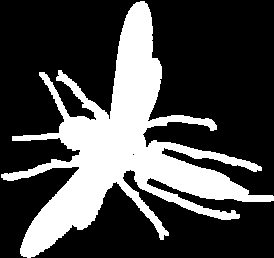
\includegraphics[scale=0.15]{Illustrations/fly-6.png} & 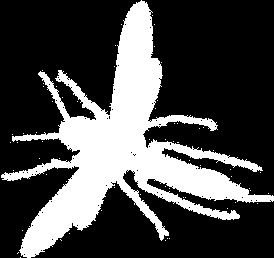
\includegraphics[scale=0.15]{Illustrations/fly-6(3).png} & 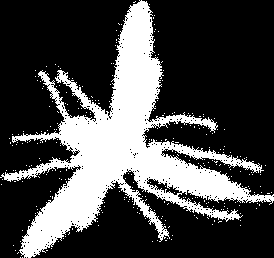
\includegraphics[scale=0.15]{Illustrations/fly-6(5).png} & 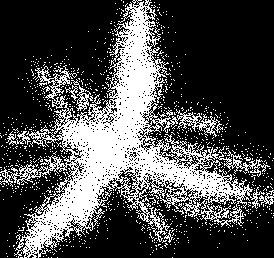
\includegraphics[scale=0.15]{Illustrations/fly-6(8).png} \\
	    \cline{2-6}
	    & Solidité & 0.65156 & 0.703824 & 0.842951 & 0.989008 \\
	    \hline
	    \hline
	    & Bruit & 0 & 0.3 & 0.5 & 0.8 \\
	    \cline{2-6}
	    Clé & Image & 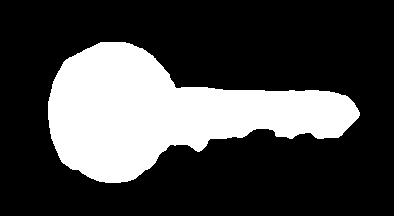
\includegraphics[scale=0.15]{Illustrations/key-6.png} & 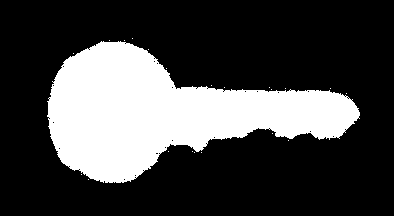
\includegraphics[scale=0.15]{Illustrations/key-6(3).png} & 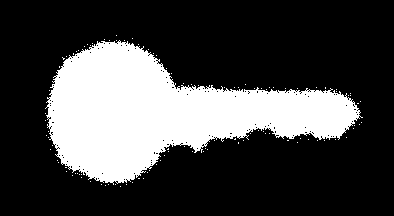
\includegraphics[scale=0.15]{Illustrations/key-6(5).png} & 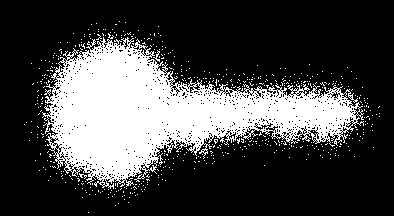
\includegraphics[scale=0.15]{Illustrations/key-6(8).png} \\
	    \cline{2-6}
	    & Solidité & 0.787878 & 0.866782 & 0.849132 & 0.985798 \\
	    \hline
	    \hline
	    & Bruit & 0 & 0.3 & 0.5 & 0.8 \\
	    \cline{2-6}
	    Serpent de mer & Image & 
\includegraphics[scale=0.3]{Illustrations/sea_snake-20.png} & 
\includegraphics[scale=0.3]{Illustrations/sea_snake-20(3).png} & 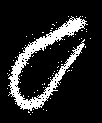
\includegraphics[scale=0.3]{Illustrations/sea_snake-20(5).png} & 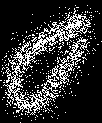
\includegraphics[scale=0.3]{Illustrations/sea_snake-20(8).png} \\
	    \cline{2-6}
	    & Solidité & 0.47619 & 0.484626 & 0.963883 & 0.959282 \\
	    \hline	    
	  \end{tabular}
	  \caption{Variations de la solidité de plusieurs objets selon le bruit}
	  \label{solidité-noise-table}
	  \end{table}
	  
	  C'est pourquoi, l'estimateur applique un traitement anti-bruit (voire Section \ref{sec:anti-bruit}) avant de faire son calcul. On peut observer, avec la Table \ref{solidité-noise-debruite-table} que les résulats sont alors bien meilleurs. En effet, la solidité reste stable tant que la valeur du bruit n'est pas trop élevée. Lorsque le bruit atteint la valeur 0.8, par contre, la solidité explose, tout comme dans le cas où l'image n'est pas débruitée avant le calcul. Cependant, on remarque que lorsque le bruit atteint de telles valeurs, l'image est alors assez déconstruite, même pour un observateur humain. Et cela est d'autant plus vrai que l'image est petite. Ce n'est donc pas si mal. \\
	  
	  \begin{table}[!h] %Si on pouvait centrer verticalement ce serait le top
	  \centering
	  \begin{tabular}{|c|c|c|c|c|c|}
	    \hline
	    & Bruit & 0 & 0.3 & 0.5 & 0.8 \\
	    \cline{2-6}
	    Mouche & Image & 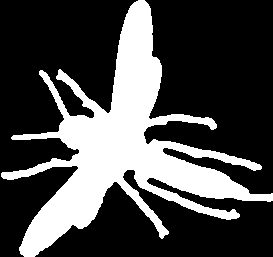
\includegraphics[scale=0.15]{Illustrations/fly-6-debruite.png} & 
\includegraphics[scale=0.15]{Illustrations/fly-6-debruite(3).png} & 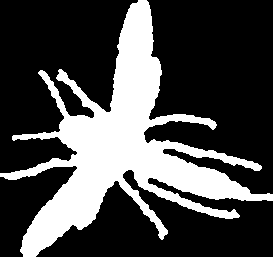
\includegraphics[scale=0.15]{Illustrations/fly-6-debruite(5).png} & 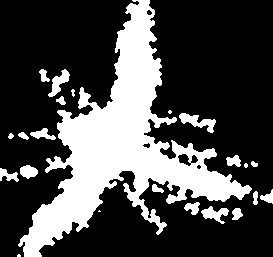
\includegraphics[scale=0.15]{Illustrations/fly-6-debruite(8).png} \\
	    \cline{2-6}
	    & Solidité & 0.652126 & 0.650744 & 0.649821 & 0.838861 \\
	    \hline
	    \hline
	    & Bruit & 0 & 0.3 & 0.5 & 0.8 \\
	    \cline{2-6}
	    Clé & Image & 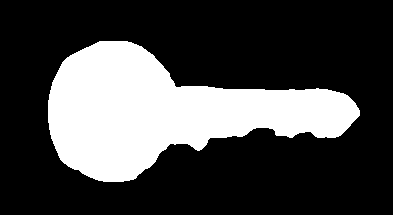
\includegraphics[scale=0.15]{Illustrations/key-6-debruite.png} & 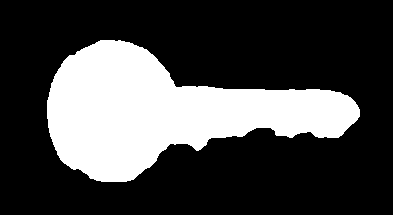
\includegraphics[scale=0.15]{Illustrations/key-6-debruite(3).png} & 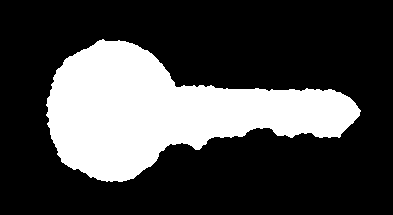
\includegraphics[scale=0.15]{Illustrations/key-6-debruite(5).png} & 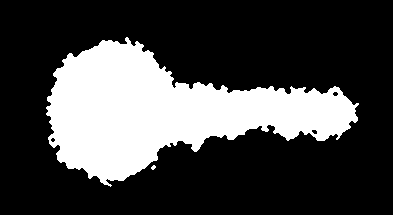
\includegraphics[scale=0.15]{Illustrations/key-6-debruite(8).png} \\
	    \cline{2-6}
	    & Solidité & 0.785436 & 0.783812 & 0.780256 & 0.735086 \\
	    \hline
	    \hline
	    & Bruit & 0 & 0.3 & 0.5 & 0.8 \\
	    \cline{2-6}
	    Serpent de mer & Image & 
\includegraphics[scale=0.3]{Illustrations/sea_snake-20-debruite.png} & 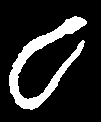
\includegraphics[scale=0.3]{Illustrations/sea_snake-20-debruite(3).png} & 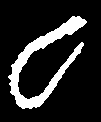
\includegraphics[scale=0.3]{Illustrations/sea_snake-20-debruite(5).png} & 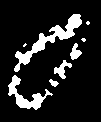
\includegraphics[scale=0.3]{Illustrations/sea_snake-20-debruite(8).png} \\
	    \cline{2-6}
	    & Solidité & 0.485542 & 0.491055 & 0.483393 & 0.960359 \\
	    \hline	    
	  \end{tabular}
	  \caption{Variations de la solidité de plusieurs objets selon le bruit, après débruitage}
	  \label{solidité-noise-debruite-table}
	  \end{table}
	  
	  Les expérimentations nous amènenet également à observer que la solidité avec ou sans débruitage diffèrent sensiblement, et ce même pour des images non bruitées. Il convient donc de construire le modèle en appliquant également le traitement anti-bruit à la base de données.

%	pour résumer :
%- quand le bruit devient vraiment important (genre 0.8), ça a tendance a foirer que ce soit debruité ou pas
%- sinon c'est plutot pas mal
%- par contre l'estimateur avec et sans débruitage sont assez loin
%=> il faut le modèle avec un traitement anti bruit


	\paragraph{Résistance aux rotations et symmétries}
	
	  L'estimateur ne tient aucun compte de l'orientation de l'image, il est donc tout à fait résistant aux rotations et aux symmétries.
      
	\paragraph{Résistance aux homothéties} 
	
	  Si on regarde la définition de la solidité, on a un estimateur qui devrait être résistant aux homothéties. Cependant comme l'agrandissement ou le rétrecissement d'une image discrète ne se comporte pas toujours comme l'intuition le commanderait, nous avons réalisé des tests pour vérifier que c'était bien le cas.
	  
	  La Table \ref{solidité-scaling-table} montre une partie représentative de ces tests. On s'aperçoit qu'effectivement la solidité reste stable par homothétie.\\
	
	  \begin{table}[!h]
	  \centering
	  \begin{tabular}{|c|c|c|c|c|c|c|c|}
	    \hline
	    \multicolumn{2}{|c|}{Cheval} & \multicolumn{2}{|c|}{Pomme} & \multicolumn{2}{|c|}{Device} & \multicolumn{2}{|c|}{Lézard} \\
	    \multicolumn{2}{|c|}{\includegraphics[scale=0.15]{Illustrations/horse-20.png}} 
	    & \multicolumn{2}{|c|}{\includegraphics[scale=0.15]{Illustrations/apple-3.png}} 
	    & \multicolumn{2}{|c|}{\includegraphics[scale=0.075]{Illustrations/device7-1.png}} 
	    & \multicolumn{2}{|c|}{\includegraphics[scale=0.09]{Illustrations/lizzard-13.png}} \\
	    \hline
	    \textbf{Echelle} & \textbf{Solidité} & \textbf{Echelle} & \textbf{Solidité} & \textbf{Echelle} & \textbf{Solidité} & \textbf{Echelle} & \textbf{Solidité} \\
	    \hline
	    0.5 & 0.584583 & 0.5 & 0.933504 & 0.5 & 0.77016 & 0.5 & 0.767554 \\
	    \hline
	    1 & 0.577491 & 1 & 0.931911 & 1 & 0.768281 & 1 & 0.762166 \\
	    \hline
	    2 & 0.57244 & 2 & 0.930546 & 2 & 0.767288 & 2 & 0.75678 \\
	    \hline
	    5 & 0.569273 & 5 & 0.929267 & 5 & 0.703692 & 5 & 0.7533 \\
	    \hline
	  \end{tabular}
	  \caption{Variations de la solidité de plusieurs objets selon l'agrandissement}
	  \label{solidité-scaling-table}
	  \end{table}
	  
	  On peut remarquer que plus l'image est grande, plus la solidité diminue, pour une même forme. Cela vient du fait que lorsqu'on agrandit l'image, les extrémités n'augmentent pas significativement l'aire de l'image, mais augmentent en revanche beaucoup plus l'aire de l'enveloppe convexe. On remarque d'ailleurs, en comparant l'évolution de la solidité de Device et celle de Lézard, que plus la forme est ``branchée'', plus sa solidité diminue rapidement en fonction de sa taille. Une idée pourrait même être de distinguer des images selon l'évolution de la solidité par homothéties de l'image. Mais cette méthode risque d'être très coûteuse.
	  
	\paragraph{Résistance aux élongations}
	
	  L'estimateur n'est pas résistant aux élongations. Cependant, l'écart de solidité entre une forme et son allongée n'est pas vraiment catastrophique. Aucune solution n'a été réellement recherchée pour résoudre ce problème.
	
	\paragraph{Résistance aux occlusions}
	  
	  De par sa nature, l'estimateur résiste très très mal aux occlusion qui vont faire diminuer drastiquement la solidité. De même que pour l'élongation, aucune solution n'a été réellement recherchée pour résoudre ce problème.
	  
	\paragraph{Résultats}

	  On peut remarquer en ragardant la Figure \ref{solidité-graph}, que la solidité ne discrimine pas beaucoup de classe. En particulier lorsqu'elle vaut environ 0.8, elle correspond à une majorité de classes. Ce n'est guère suprenant venant d'un estimateur aussi simple qui réduit une forme complexe à un scalaire. \\
	  
	  \begin{figure}[!h]
	    \begin{bigcenter}
	      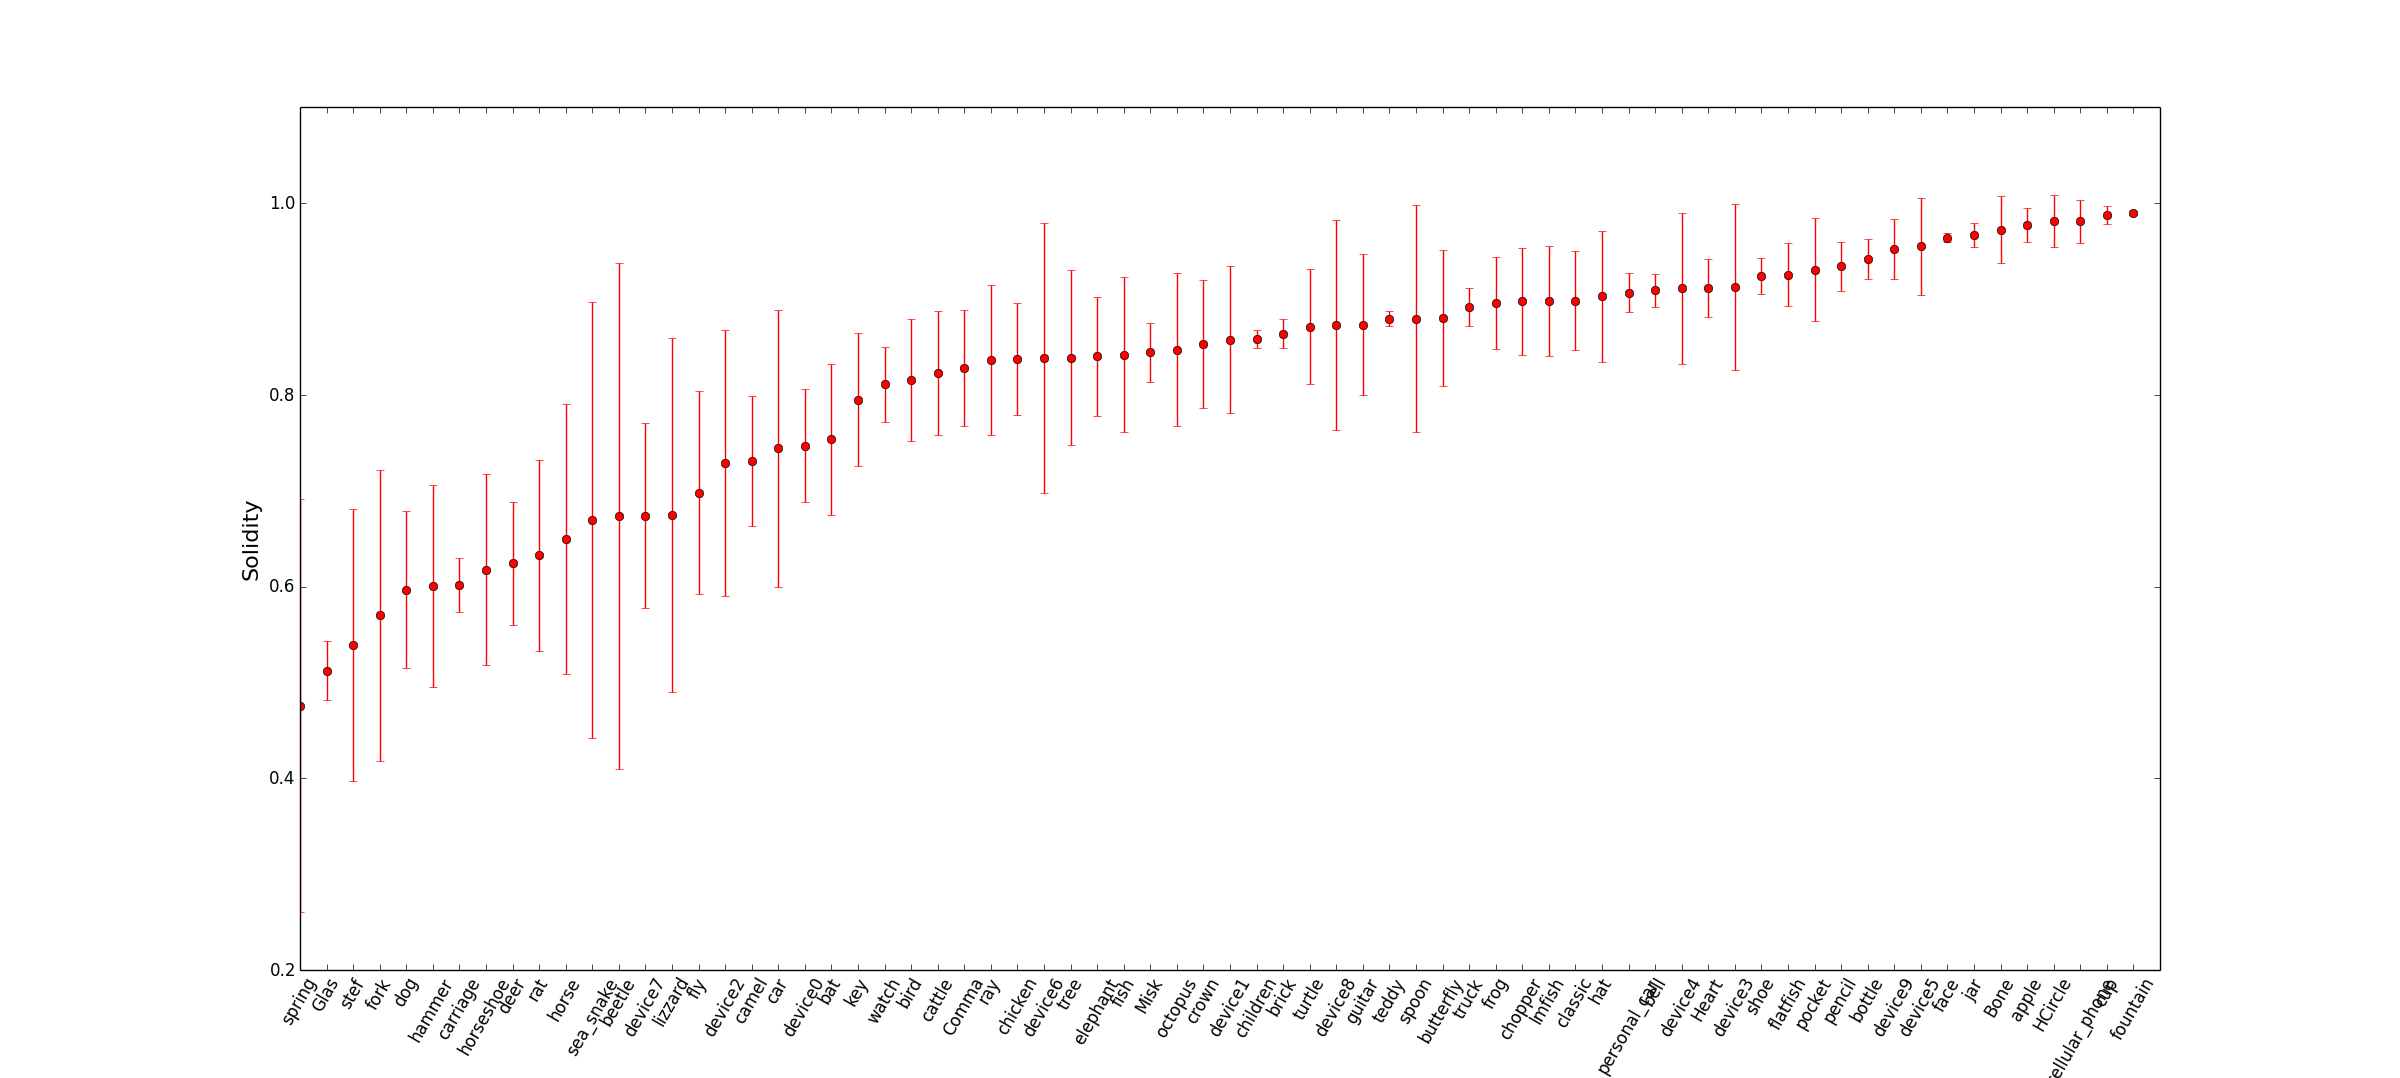
\includegraphics[scale=0.38]{Graphes/solidite.png}
	    \end{bigcenter}
	    \caption{Moyenne et écart type de la solidité pour chaque classe}
	    \label{solidité-graph}
	  \end{figure}
	  
	  En revanche cet estimateur semble être relativement pertinent pour un certain nombre de classes, on peut donc espérer qu'en le couplant avec d'autres estimateurs les résultats seront satisfaisants.  

      \subsubsection{Excentricté}
      
	\paragraph{Principe}
	
	  L'idée de l'xcentricité d'une forme est d'adapter la notion intuitive d'excentricité d'une ellipse à une forme plus complexe. Il y a plusieurs manière de définir l'excentricité pour une forme quelconque. Celle que nous avons choisie a l'avantage d'être facile à implémenter. Elle s'interprète comme un indicateur de l'alongement de la forme.
	  
	  \begin{definition}[Excentricité]
	    On appelle excentricité le rapport de la longueur sur la largeur du rectangle à limite minimum de la forme.
	  \end{definition}
      
	\paragraph{Programmation}
	
	  Pour calculer l'excentricité d'une forme, on procède de la façon suivante :
	  \begin{itemize}
	   \item On calcule la distance maximale entre deux points de la forme. Cette distance sera la longueur du rectangle à limite minimum de la forme.
	   \item On pivote l'image de façon à ce que la longeur du rectangle se retrouve à être l'horizontale (par un simple calcul d'angle). De cette manière, la direction perpendiculaire à la longueur est la verticale.
	   \item A partir de là, on trouve facilement la largueur en parcourant verticalement l'image et en retenant la distance verticale maximum entre deux points de l'image.
	  \end{itemize}
	
	\paragraph{Résistance aux inversions de couleur}
	
	  Comme ce n'est réellement que les contours de la forme qui sont étudiés, l'estimateur en lui-même est résistant aux inversions de couleurs. Cependant il a été codé de manière à fonctionner lorsque les images sont blanches sur fond noir. Il est donc nécessaire d'appliquer un traitement anti-inversion (voire Section \ref{sec:anti-inversion}) avant de faire le calcul.
	
	\paragraph{Résistance au bruit}
	
	  Le rectangle à limite minimum de la forme est assez peu sensible au faible bruit. De plus, même si le fort bruit risque de faire s'agrandir ce rectangle, le rapport longueur sur lareur ne change pas sensiblement car la dispersion est a priori isotrope. Les tests effectués et figurant Table \ref{excentricité-noise-table}, nous confirment ce fait. \\
	
	  \begin{table}[!h] %Si on pouvait centrer verticalement ce serait le top
	  \centering
	  \begin{tabular}{|c|c|c|c|c|c|}
	    \hline
	    & Bruit & 0 & 0.3 & 0.5 & 0.8 \\
	    \cline{2-6}
	    Mouche & Image & 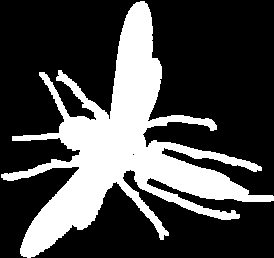
\includegraphics[scale=0.15]{Illustrations/fly-6.png} & 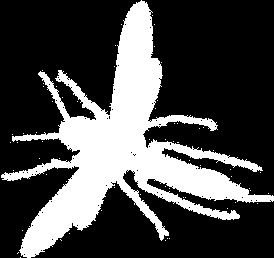
\includegraphics[scale=0.15]{Illustrations/fly-6(3).png} & 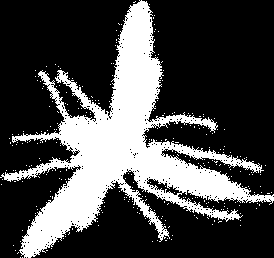
\includegraphics[scale=0.15]{Illustrations/fly-6(5).png} & 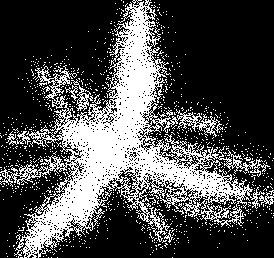
\includegraphics[scale=0.15]{Illustrations/fly-6(8).png} \\
	    \cline{2-6}
	    & Excentricité & 1.37561 & 1.42 & 1.37681 & 1.37383 \\
	    \hline
	    \hline
	    & Bruit & 0 & 0.3 & 0.5 & 0.8 \\
	    \cline{2-6}
	    Clé & Image & 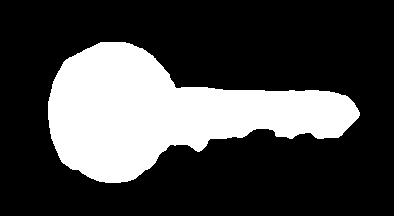
\includegraphics[scale=0.15]{Illustrations/key-6.png} & \includegraphics[scale=0.15]{Illustrations/key-6(3).png} & \includegraphics[scale=0.15]{Illustrations/key-6(5).png} & \includegraphics[scale=0.15]{Illustrations/key-6(8).png} \\
	    \cline{2-6}
	    & Excentricité & 2.22143 & 2.19718 & 2.09934 & 2.04023 \\
	    \hline
	    \hline
	    & Bruit & 0 & 0.3 & 0.5 & 0.8 \\
	    \cline{2-6}
	    Serpent de mer & Image & \includegraphics[scale=0.3]{Illustrations/sea_snake-20.png} & \includegraphics[scale=0.3]{Illustrations/sea_snake-20(3).png} & \includegraphics[scale=0.3]{Illustrations/sea_snake-20(5).png} & \includegraphics[scale=0.3]{Illustrations/sea_snake-20(8).png} \\
	    \cline{2-6}
	    & Excentricité & 1.1383 & 1.14894 & 1.16842 & 1.05426 \\
	    \hline	    
	  \end{tabular}
	  \caption{Variations de l'excentricité de plusieurs objets selon le bruit}
	  \label{excentricité-noise-table}
	  \end{table}
	  
	  Des tests ont également été éffectués après un débruitage des objets, et on a pu remarquer que la stabilité de l'excentrité était un peu près la même.
	
	\paragraph{Résistance aux rotations et symmétries}
      
	  Tout comme le calcul de la solidité, l'estimateur ne tient aucun compte de l'orientation de l'image, il est donc tout à fait résistant aux rotations et aux symmétries.
      
	\paragraph{Résistance aux homothéties} blabla
	
	  Si on regarde la définition de lexcentricité, on a un estimateur qui devrait être complètement résistant aux homothéties. En effet, lorsqu'on agrandit la forme, on agrandit d'autant le rectangle à limite minimum de la forme, mais le rapport longueur sur largeur de ce rectangle reste invariant. Des tests ont été conduits pour vérifier que c'était bien le cas.
	  
	  La Table \ref{solidité-scaling-table} montre une partie représentative de ces tests. On s'aperçoit qu'effectivement l'excentricité reste stable par homothétie.\\
	
	  \begin{table}[!h]
	  \centering      
	  \begin{tabular}{|c|c|c|c|c|c|}
	    \hline
	    \multicolumn{2}{|c|}{Chauve-souris} & \multicolumn{2}{|c|}{Marteau} & \multicolumn{2}{|c|}{Device}  \\
	    \multicolumn{2}{|c|}{\includegraphics[scale=0.11]{Illustrations/bat-2.png}} 
	    & \multicolumn{2}{|c|}{\includegraphics[scale=0.15]{Illustrations/hammer-20.png}} 
	    & \multicolumn{2}{|c|}{\includegraphics[scale=0.07]{Illustrations/device9-9.png}}  \\
	    \hline
	    \textbf{Echelle} & \textbf{Excentricité} & \textbf{Echelle} & \textbf{Excentricité} & \textbf{Echelle} & \textbf{Excentricité} \\
	    \hline
	    0.5 & 2.32927 & 0.5 & 2.92308 & 0.5 & 1.0101 \\
	    \hline
	    1 & 2.33841 & 1 & 2.89873 & 1 & 1.01515 \\
	    \hline
	    2 & 2.33994 & 2 & 2.91772 & 2 & 1.01641 \\
	    \hline
	    5 & 2.34065 & 5 & 2.92152 & 5 & 1.01767 \\
	    \hline
	  \end{tabular}
	  \caption{Variations de l'excentricité de plusieurs objets selon l'agrandissement}
	  \label{excentricité-scaling-table}
	  \end{table}  
	  
	\paragraph{Résistance aux élongations}
	
	  De par sa nature, l'estimateur résiste très très mal aux élongations qui vont faire augmenter drastiquement l'excentricité. Aucune solution n'a été réellement recherchée pour résoudre ce problème.
	
	\paragraph{Résistance aux occlusions}
	  
	  L'estimateur est relativement résistant aux petites occlusions qui n'empiètent pas sur toute une partie de la forme. Cependant il résiste très mal aux occlusions plus sévères. Aucune solution n'a été réellement recherchée pour résoudre ce problème.
	  
	\paragraph{Résultats}
	
	  Lorsqu'on calcule la moyenne et l'écart type de l'excentricité pour chaque classe (représenté Figure \ref{eccentricity-graph}), ce qui frappe est que l'estimateur semble pertinent pour la plupart des classes, mais que pour quelques unes il donne des valeurs aberrantes. En ragardant la base de donnée, on s'aperçoit que c'est dans des cas où il y a de l'élongation. L'exemple typique est la classe \texttt{pocket} dont l'écart type est 19 pour des valeurs qui vont habituellement de 0 à 5. Or la classe \texttt{pocket} regroupe des images de montres qui sont vues de face, sauf dans le cas d'une qui est vue de côté (voire Figure \ref{class-pocket}).  \\
	
	  \begin{figure}[!h]
	    \begin{bigcenter}
	      \includegraphics[scale=0.38]{Graphes/eccentricity.png}
	    \end{bigcenter}
	    \caption{Moyenne et écart type de l'excentricité pour chaque classe}
	    \label{eccentricity-graph}
	  \end{figure}
	  
	  \begin{figure}[!h]
	    \centering
	    \begin{subfigure}{.2\textwidth}
	      \centering
	      \includegraphics[scale=0.25]{Illustrations/pocket-20.png}
	    \end{subfigure}
	    \begin{subfigure}{.2\textwidth}
	      \centering
	      \includegraphics[scale=.9]{Illustrations/pocket-9.png}
	    \end{subfigure}
	    \begin{subfigure}{.15\textwidth}
	      \centering
	      \includegraphics[scale=0.235]{Illustrations/pocket-14.png}
	    \end{subfigure}
	    \caption{Les objets de la classe \texttt{pocket}}
	    \label{class-pocket}
	  \end{figure}
	  
	  Si on zoome un peu sur les valeurs intéressantes du graph présenté Figure \ref{eccentricity-graph}, on observe que les valeurs ne sont pas aussi rammasées qu'on aurait pu le croire au premier coup d'oeil. L'excentrité discrimine bien les classes, du moins pour un estimateur aussi simple, et a l'air d'être un bon complémentaire à solidité.
	  
	  \begin{figure}[!h]
	    \begin{bigcenter}
	      \includegraphics[scale=0.38]{Graphes/eccentricitybis.png}
	    \end{bigcenter}
	    \caption{Moyenne et écart type de l'excentricité pour chaque classe}
	    \label{eccentricity-graph-2}
	  \end{figure}
      
      \subsubsection{Energie de flexion moyenne}
      
	\paragraph{Principe}
	
	\paragraph{Programmation}
	
	  Méthode du cercle circonscrit par les deux demis tangentes.
	  
	  \begin{figure}[!h]
	    \centering
	    \begin{tikzpicture}
	    \begin{scope}[scale = .4]
	      \draw (0,0) circle (5);
	      \node[] at (30:5) (Q) {\textbullet};
	      \node[right=.01cm of Q] {$Q$};
	      \node[] at (80:5) (P) {\textbullet};
	      \node[above=.01cm of P] {$P$};
	      \node[] at (165:5) (O) {\textbullet};
	      \node[left=.01cm of O] {$O$};
	      \draw[] (30:5) -- (80:5) -- (165:5) -- (30:5);
	      \node[] (C) {$\times$};
	      \node[below right=.01cm and .01cm of C] {$C$};
	      \draw[dashed] (0,0) -- node[right]{$r$} (80:5);
	    \end{scope}
	    \end{tikzpicture}
	    \caption{Cercle circonscrit au triangle OPQ}
	    \label{cercle-circonscrit}
	  \end{figure}
	  
	  Par la loi des sinus, $r = \frac{|QO|}{2 \sin\left(\widehat{OPQ}\right)}$. On en déduit que :
	  
	  \[ r = \frac{|QO|}{2 \sin\left(\widehat{OPQ}\right)} = \frac{|QO|}{\frac{2 \det\left(\overrightarrow{PO}, \overrightarrow{PQ} \right)}{|OP| |PQ|}} = \frac{|OP| |PQ| |QO|}{4 \mathcal{A}_{PQO}}  \]
	
	\paragraph{Résultats}
  
    
    \subsection{Méthode des moments} %A renommer ? Raphaël
      Cet estimateur est simple d'où son nom d'exécutable \verb-libbasicestim-. On reprend l'idée de la normalisation d'image évoquée plus haut.
      
      Notons $S$ l'ensemble des points de l'objet, $|S|$ son cardinal, $G$ son centre de gravité et $d(A,B)=||A-B||_2$ la distance entre deux points.
      
      On calcule $m=\frac{\sum_{P\in S}d(P,G)}{|S|}$ la distance moyenne à $G$ et $v=\sqrt{\frac{\sum_{P\in S}\left ( d(P,G) -m\right ) ^2}{|S|}}$ l'écart-type.
      
      Afin de pouvoir comparer ces grandeurs, on les norme par l'écart maximal entre un point de $S$ et $G$.
      
      Ces deux valeurs constituent les grandeurs caractéristiques de l'estimateur.
      
      L'estimateur est ainsi naturellement résistant aux rotations, aux translations et à l'agrandissement. Statistiquement, il est insensible au bruit pour la moyenne, ainsi que pour l'écart type dans une certaine mesure.
    
    \subsection{Etude du squelette} %TODO : Raphaël
    
    Le squelette de l'objet pourrait apporter beaucoup d'informations. Cependant ici on se concentrera sur ce que l'on appelle la colonne vertébrale définie comme plus grand chemin dans le squelette. Cette information est pertinente dans le sens où cela peut caractériser la longueur de l'objet une fois ``déplié''. Pour donner un sens à cela on normalisera d'abord l'image comme décrit dans le traitement normalisation. On débruitera aussi l'image pour que le squelette soit ``naturel''. On rempliera la forme pour que le squelette soit un arbre. Si la forme n'est pas connectée, on ne gardera que le plus grand arbre restant
    
    Ici le squelette sera calculé par effeuillages successif du contour de l'objet.
    
     \begin{figure}[!h]
	\centering
	\begin{subfigure}{.45\textwidth}
	  \centering
	  \includegraphics[scale=0.25]{Illustrations/turtle.png}
	  \label{pocket-non-rempli}
	\end{subfigure}
	\begin{subfigure}{.45\textwidth}
	  \centering
	  \includegraphics[scale=0.25]{Illustrations/turtlesk.png}
	\label{pocket-rempli}
	\end{subfigure}
	\caption{L'image de tortue normée et son squelette}
	\label{skelton}
      \end{figure}
      
      La longueur de la colonne vertébrale est par normalisation invariante à l'agrandissement. Elle est naturellement invariante par rotation et translation. Comme il y a un débruitage elle est résistante au bruit et de toute façons comme on prend la branche de longueur maximale, des branches artéfacts ne sont pas si gênantes.
    
    \subsection{Pistes non explorées}
        \subsubsection{Transformée de Fourier} 
        
        Utiliser la transformée de Fourier pour obtenir le spectre semble un bon moyen de caractériser une image. Surtout que supprimer le bruit reviendrait à négliger les hautes fréquences. La transformée es invariante par translation si on ne s'intéresse qu'à l'amplitude des différentes fréquences. On peut la rendre invariante par rotation en se plaçant au centre de gravité et en utilisant les coordonnées polaires
        
        Pour comparer les spectres l'Earth mover's distance semble être appropriée (cependant en réduisant la taille des images à $64 \times 64$ le nombre de point est beaucoup trop gros pour résoudre l'instance par une relaxation linéaire)
        
        \subsubsection{Comparaison de squelette}  %A mettre ? RAphaël
        
        Comparer des graphes serait trop ambitieux car ce genre de problème (comme l'isomorphisme) est NP-Complet. Cependant, comme vu plus le squelette est ici un arbre. Donc la comparaison semble possible en temps raisonnable. L'idée serait de voir le cout minimal des opérations pour passer d'un squelette à un autre avec les opérations élémentaires : allonger une branche, rajouter une branche.
  
  \section{Résultats} 
  
    \subsection{Méthodologie d'estimation}  %En gros : c'est quoi nos résultats ?, je sais pas trop comment le nommer
    
    \subsection{Résultats} %Beaucoup de section / subsection = résultats
  
  \section{Conclusion}
  
\end{document}

